In questo esperimento si vuole costruire e studiare un amplificatore in classe B, realizzato tramite push-pull. Il circuito è riportato in Figura \ref{fig:Circuit2}.
\begin{figure}[H]
    \centering
    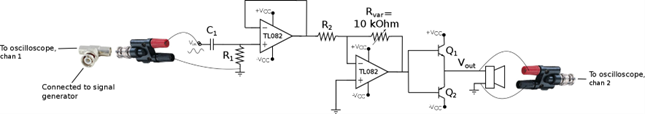
\includegraphics[width=\linewidth]{images/Circuit2.png}
    \caption{Schema circuito}
    \label{fig:Circuit2}
\end{figure}
Il circuito è alimentato dalla tensione duale: $\pm V_{CC}=\pm3V$.\\\\
Il funzionamento per i primi 2 stadi è uguale a quanto detto nel Paragrafo \ref{ch:Spiegazione1}, mentre lo stadio di uscita permette di avere un rendimento migliore di quello ottenuto nell'esperienza precedente. L'efficienza di questo tipo di stadio è dovuta all'attivazione di un solo transistor per semionda. Tuttavia, come si vedrà successivamente, questo circuito ha l'inconveniente di una sensibile distorsione di crossover, dovuta alla soglia di conduzione dei transistor.
\subsection{Assemblaggi e settaggi}
Il circuito in Figura \ref{fig:Circuit2} è stato realizzato modificando direttamente lo schema in classe A (Figura \ref{fig:Circuit1}) con uno stadio in classe B e sostituendo l'integrato MCP6002 con l'integrato TL082CP.\\\\
Lo stadio in classe B push-pull è stato realizzato utilizzando l'accoppiamento di un transistor di potenza NPN $(Q_1)$, codice TIP41CG e un transistor PNP di potenza $(Q_2)$, codice TIP42CG. Le altre componenti sono rimaste invariate dal Primo esperimento\\\\
Il generatore di forma d'onda è stato impostato con il seguente segnale:
\begin{itemize}
    \item Forma d'onda: sinusoidale
    \item Ampiezza iniziale: $100mV$ picco-picco
    \item Frequenza: $330Hz$ (nota Mi)
\end{itemize}
\clearpage
\subsection{Procedura di valutazione e risultati}
Dopo aver acceso l'alimentazione, l'oscilloscopio è stato impostato in modo da visualizzare il segnale di ingresso e il segnale di uscita. Il potenziometro che regola il volume è stato regolato in modo di raggiungere un'ampiezza di $1V_{pp}$ sul segnale di uscita.\\
Si è proseguito a misurare i due segnali con l'oscilloscopio, le cui forme d'onda sono riportare in Figura \ref{fig:scope_9} 
\begin{figure}[H]
    \centering
    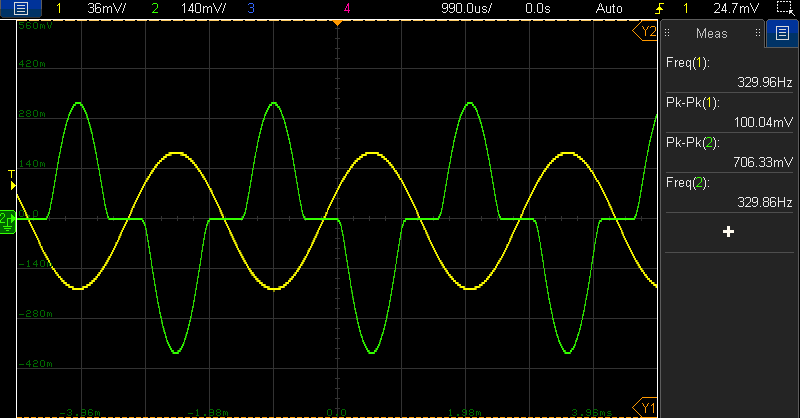
\includegraphics[width=0.7\linewidth]{images/scope_9.png}
    \caption{Segnali di ingresso e uscita dell'amplificatore in classe B}
    \label{fig:scope_9}
\end{figure}
Si è proseguito misurando, attraverso i cursori dell'oscilloscopio, il tempo morto dovuto alla distorsione di crossover.
\begin{equation*}
    \text{Dead time} = 503.125\mu s
\end{equation*}
risultato piùttosto rilevante, considerato che la forma d'onda data in ingresso ha periodo di $T=3\text{ms}$. Si riporta in Figura \ref{fig:scope_11} il dettaglio della distorsione di crossover
\begin{figure}[H]
    \centering
    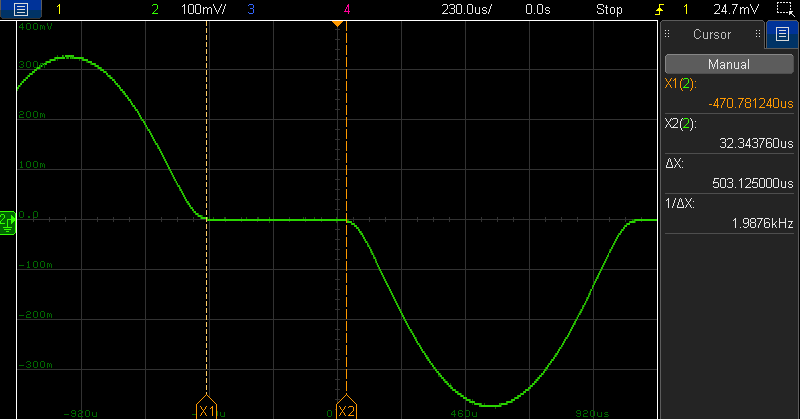
\includegraphics[width=0.7\linewidth]{images/scope_11.png}
    \caption{Dettaglio misurazione distorsione crossover}
    \label{fig:scope_11}
\end{figure}
\subsubsection{Lettore MP3}
Come spiegato nella prima esperienza, si deciso di utilizzare una resistenza di 8$\Omega$ al posto dell'altoparlante, quindi non si è potuto svolgere la prova della riproduzione di una traccia audio. L'obiettivo era quello di sentire l'effetto della distorsione di crossover.
\subsubsection{Commenti}
Le prestazioni di questo amplificatore sono buone, anche se con qualche compromesso. Infatti a livello teorico il rendimento è molto alto, ci sono poce dispersioni di potenza. Come contro, questo circuito ha una distorsione del segnale di uscita decisamente elevata.